\chapter{Memristive Properties of Nanowire Networks}
Until now, the conductive properties of a NWN have been examined for static nanowire junctions that have been annealed in some manner into a low resistance state. The surface layer in individual nanowires - a polymer, native oxide or some other surfactant - are a necessity to stabilise the nanowires during synthesis\cite{shah2004}. Surface layers act as an insulating barrier between the highly conductive metallic cores of the nanowires which has traditionally been seen as an undesirable feature in NWNs that are incorporated in transparent conductor devices, as a minimal resistance is required for many applications\cite{mutiso2013}. In fact, the preceding two chapters had a large focus on understanding the effect of junction resistance on annealed NWNs and their upper-limit sheet conductance where the inter-wire junctions are annealed to low values. The potential exploitation of these insulating, unannealed barriers has thus gone largely unexplored.

A popular annealing method for NWNs is electrical stressing\cite{rocha2015,bellew2015}, where an applied current is gradually increased from small current ranges until the resistance of the NWN is decreased, but not so high as to cause wire failures due to melting from Joule heating\cite{lagrange2016,zhao2011}. Nirmalraj et al showed that electrical annealing can be controlled to tune the conductivity of a NWN, gradually increasing the connectivity of the NWN by increasing the annealing current flow\cite{nirmalraj2012}. This gradual increase in NWN conductivity is akin to a class of materials known as memristors (memory resistors) that were introduced in chapter 1. As discussed in chapter 1, memristors were first hypothesised in 1971 by Chua and their defining behaviour is a non-constant, non-linear, reversible resistance that is mediated by some tunable internal state variable\cite{chua1971}. The internal state variable corresponds to some physical phenomenon that can be controlled via some external means. For example, many memristors are mediated by an ion-doped layer or a conductive filament, the size of which is controlled by current-flow to cause various resistance states\cite{strukov2008,waser2007,valov2011}. Since the first experimental realisation of a memristor in 2008\cite{strukov2008}, many examples of memristors have been demonstrated, one such device is a planar metal-insulator-metal (MIM) tri-layer junction. The MIM architecture that is common in memristors are found in un-annealed nanowire junctions, the metals being the cores of the NWNs and the two surface layers acting as the insulating barrier, a sketch of such a system is given in Figure \ref{fig: filament_sketch}. This means that a NWN contains many highly connected MIM junctions, and offers a rich new area of potential applications as memristive and neuromorphic (brain-like computing) devices. In chapter 1, in a discussion of Ag MIM junctions, it was shown how a conductive filament forms between electrodes and mediates the memristive response of the device\cite{yang2012}. In Ag/PVP nanowire junctions, a conductive filament should also mediate their memristance\cite{scaling2018}, and is depicted between metallic cores in Figure \ref{fig: filament_sketch}.

\fig{1}
{Images/Chapter5/filament_sketch.pdf}
{\textbf{Sketch:} Sketch of a conductive filament formed between two core-shell nanowires.}
{Sketch of a conductive filament formed between the metallic cores (silver) of two intersecting Ag/PVP nanowires. The shaded blue regions represent the insulating shells of the nanowires, and the system as a whole is viewed along the direction of the bottom nanowire.}
{fig: filament_sketch}

To date, there has been numerous attempts to mimic biological computation through simulations on traditional von Neumann computer architectures \cite{indiveri2013}. However, this approach is computationally expensive due to von Neumann bottlenecks, essentially the limit of how quickly data can be moved from memory to a processing unit in a computer. Another approach to achieve biological computation is through the use of neuromorphic computing architectures\cite{prezioso2015,yang2013}. These can be decentralised networks of memristor units capable of mimicking analogue synapses. While these architectures are much more energy efficient, the fabrication of such devices can be quite difficult, often requiring exact engineering of individual memristor components and connections. A high level of component homogeneity and regularity in neuromorphic networks may not be required as the variability, stochasticity, and component reliability which are becoming increasingly difficult to improve in traditional computing technologies do not pose as big a problem to biological computing systems\cite{querlioz2013}. Indeed the variability of individual synapses and the complexity of the global synapse network are exploited to perform robust and reliable computations, all while using a fraction of the power that a von Neumann computer would need for similar performance. The spacial stochasticity of the NWN coupled with the memristive properties of inter-wire junctions results in a random memristor network that is capable of performing neuromorphic computations. The random connectivity may actually be beneficial for memory storage and neuromorphic computing as a highly connected NWN has no hierarchical structure and thus should have a high fault-tolerance, a topic that is examined in chapter 6.

The aim of this chapter is to introduce a memristive model for nanowire junctions, and to report results of a computational routine that simulates the properties of a NWN with a memristive response. This goal is motivated by recent experiments that reported a memristive response of individual nanowire junctions and NWNs\cite{bellew2014,scaling2018,manning2017}; some relationships were noted between junction and network memristance that required a computational model to fully explain them\cite{scaling2018}. The layout of this chapter is as follows: experimental evidence for a memristive response of individual nanowire junctions, and a global memristive response of a NWN is presented in section \ref{Sec: mrm_model}. An empirical model for individual junctions is also introduced in this section. In section \ref{Sec: mrm_network}, a computational routine to simulate a large network of memristive junctions is introduced and the memristive responses of a network to increasing current-flow are presented. The conductance of both junctions and nanowire networks are shown to scale as a power-law with increasing current levels in section \ref{Sec: mrm_network}. The exponent of the network's power-law is shown to be the same as the individual junctions, revealing a self-similarity between the individual and the collective. The activation patterns of nanowire networks is shown to vary according to certain measurable parameters of the memristive junction model. In section \ref{Sec: current_colour}, a mapping technique is presented that allows for the visualisation of current flow through a network at any stage in its junction evolution and shows that for certain nanowire parameters the current flows through a single pathway between electrodes in a winner-takes-all manner. The existence of localised current flows has potential application in neuromorphic computing, and as a method to achieve independent and associative conductive states in a NWN is presented in section \ref{Sec: multi_terminal}. Finally a chapter summary is presented in section \ref{Sec: mrm_conclusion}

\begin{comment}
The memristive response of a number of core-shell NW juncitons have been recorded. Figure ... presents the conductance of several Ag Nw juncitons as the current compliance of the junction is gradually increasesd, i.e. as they are electrically annealed\cite{scaling2018}. There is a clear power-law relationship between the conductance and current flow, the exponent of which appears near identical for each. This power law scaling an individual junctions conductance ($\Gamma_j$) is formalised as
\begin{equation}
\Gamma_j = A_j I^{\alpha_j}
\label{eq: scaling_first}
\end{equation}
where the prefactor $A_j$ and exponent $\alpha_j$ capture the behaviour of junctions. Alongside the conductance scaling of junctions the same experiment was performed on a NWN comprised of the same AG-PVP nanowires and its conductance versus current compliance scaling is shown. Similar to the junctions, the NWN scales as a power law initially, with an exponent similar to that of the NW junctions. A richer behaviour is observed in the NWN however with a plateau appearing in the conductance scan corresponding to a period of Ohmic response of the NWN. 

Figure ... is the scaling behaviour for AG-PVP nanowire junctions and a NWN only. Further to this a number of other nanowire junctions and networks were probed in the same manner and were shown to have a conductance scaling that follows equation \ref{eq: scaling_first}. A characteristic prefactor and exponent unique to each core-shell composition were identified. These scaling parameters are outlined in Table ... The exponent for each material has a value near 1 but there is a clear distinction of sub-linear and supra-linear scaling materials. The exponents and prefactors for NWNs comprised of the Nanowires whos junctions were characterised were also determined and are given in Table ... Of particular interest is similarity of the networks exponent and the junctions exponent suggesting that a self-similar scaling between junctions and networks of junctions. 

\todo{get data/info for other wire materials. Actually fit the data}
\begin{figure}[htbp]
\centering
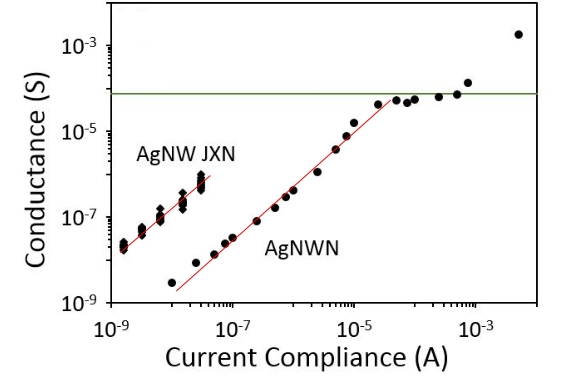
\includegraphics[width= 0.49 \columnwidth]{Images/Chapter5/exp_measurements.jpg}
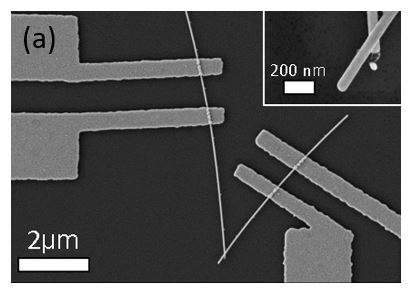
\includegraphics[width= 0.49 \columnwidth]{Images/Chapter5/single_jxn.JPG}
\caption{\fontsize{12pt}{11pt}\selectfont \textit{a) The results of recording conductance Vs current compliance for a NWN and an individual nanowire junction. An example of the experimental set-up to record the conductance of a single junction is shown in b). (c) get an image of the NWN.}}
\label{fig: exp_scaling}
\end{figure}


We assume that the conductance of each junction is bounded between the high resistance state ($10^4 k \Omega$) and the low resistance state ($13 k \Omega$). The low resistance state corresponds to $1/\Gamma_0$, where $\Gamma_0$ the quantum of conductance. Upon formation of an unbroken filament across the dielectric barrier between nanowires the width of said filament will be one atom wide. The conductance of a one atom wide wire is calculated as the quantum of conductance or $\Gamma \approx 7.75 10^{-5} S$. Individual nanowire junctions can reach the quantum of conductance at sufficiently high current levels. 

The parameter phase space for junction scaling fall into three main groups, supra-linear scaling ($\alpha_j > 1$), linear ($\alpha_j = 1$), and ($\alpha_j > 1$) sub-linear scaling ($\alpha_j < 1$). Figure BLAH shows the results of simulations with varying exponents and prefactors. The scaling exponent has a marked impact on the evolution of NWN conductance. The scaling of NWNs closely matches the scaling of individual junctions. 
\todo{image of different exponents and prefactors for same NWN.}
Effect of prefactor, the amount of current that can flow through a matured junction.

\section{Memristive Model}
In 1971 Leon Chua proposed a new circuit element known as the memristor, an element whos resistance depended on a set of state variables. The memristors behaviour is generalised with the expressions
\begin{align}
v &= \mathcal{R}(w,i)i \nonumber \\
\frac{dw}{dt} &= f(w,i) \label{eq: chua_memristor}
\end{align}
where $w$ is a set of state variables and $f$, $\mathcal{R}$ are general functions and can explicit functions in time. A rich population of theoretical memristors can be described that follow this general definition of a memristor. In their seminal paper Strukov et al presented a theoretical model for a system where its memristance is determined by an ion drift mechanism\cite{strukov2008}. The memristive characteristics of the model were similar to experements on a $TiO_x$ memristor where the change in resistance was modulated by the drift of Oxygen vacancies into a junction from a doped $TiO_{2-x}$ layer towards the undoped $TiO_2$ layer at the opposite end of the junction. The model used to describe this behaviour was
\begin{align}
V(t) & = \left[ R_{on} \frac{w(t)}{D} + R_{off}\left(1-\frac{w(t)}{D}\right) \right] I(t) \nonumber \\
\frac{dw}{dt} & = \mu_v \frac{R_{on}}{D}I(t)
\end{align}
where t is time, D is the width of the junction, $\mu_v$ is the ion mobility, I is the current through the device and V is the potential across the device. w(t) is a state variable and essentially represents the length of the doped part of the connecting junction, when $w(t) = D$ the system is in the low resistance state ($R_{on}$) and is in the high resistance state when $w(t) = 0$. 



Here the conductance scaling relationship in equation ... has been re-written in the usual format of memristors, showing that the derivative of the state variable of the CF length (w(t)) can be written as a general function of the junctions parameters.
\end{comment}
%============================================
\section{Modelling the Memristive Response of a Nanowire Junction}
\label{Sec: mrm_model}

Figure \ref{fig: exp_scaling}(a) presents experimental measurements of the conductance of individual Ag/PVP nanowire junctions for increasing current compliance, explained in chapter 1, as triangular data points. Also plot in Figure \ref{fig: exp_scaling}(a) is the conductance of an Ag/PVP NWN as circular data points\cite{scaling2018}. Here both the individual junctions and the NWN respond in a memristive manner to increasing current compliance, and these measurements reveal that their conductivity increases in a power law manner. The NWN scales with a power law over three decades of current compliance signified by the red line through the data points. Remarkably, the fitted power law to the NWN has the same exponent as the power laws fitted to the individual nanowire junctions, meaning their respective conductances ($\Gamma_{nt}$ and $\Gamma_{j}$) scale in a self-similar manner. The scaling of an individual junction is described with the power law
\begin{equation}
\Gamma_j = A_j I^{\alpha_j}
\label{eq: junction_pl}
\end{equation}
where the values of $A_j$ and $\alpha_j$ are material dependent and determine the memristive response of the material. While the memristive scaling presented in Figure \ref{fig: exp_scaling}(a) is particular to Ag/PVP nanowires, the self-similar scaling between junctions and networks was seen for a range of nanowire materials: Ni/NiO, core-shell Ag/TiO$_2$ and Cu/CuO\cite{scaling2018}. 

\fig{1}
{Images/Chapter5/exp_evidence.pdf}
{\textbf{Plot:} Conductance of a nanowire junction and network versus increasing current compliance.}
{(a) Experimental measurements of the conductance of individual Ag/PVP nanowire junctions (triangles) and an Ag/PVP NWN with increasing current compliance levels. Both systems display a power law scaling of the conductance; in the case of the NWN, this holds until a point at which the conductance reaches a plateau. (b) A magnified view of the memristive response of the NWN in (a) in the vicinity of the plateau where the conductance of the network $\Gamma_{nt}$ has been normalised by the quantum of conductance $\Gamma_0$. Here several smaller plateaus are observed with a conductance $\Gamma_p$ that are fractions of $\Gamma_0$\cite{scaling2018}. }
{fig: exp_scaling}

Another intriguing phenomenon is observed in the NWN conductance curve where it no longer scales as a power law and reaches a plateau. Figure \ref{fig: exp_scaling}(b) is a magnified view of this region where the fine detail can be seen. Three distinct plateaus in the network conductance can be seen, each represented by the horizontal orange and brown lines. The conductance of the network has been normalised by the quantum of conductance ($\Gamma_0 = 2 e^2/h$), the conductance of a single atomic channel that can transport a single spin degenerate pair of electrons, where $e$ is the charge of an electron and $h$ is Planck's constant. The plateaus have an approximate normalised conductance of $\Gamma_{nt}/\Gamma_0 \approx 1/8$ (bottom), $\Gamma_{nt}/\Gamma_0 \approx 1/6$ (middle), and $\Gamma_{nt}/\Gamma_0 \approx 1/5$ (top). Conductance plateaus were not seen for all of the examined NWN materials mentioned above meaning that specific material properties are required to observe them. In this section, a memristive model for individual nanowire junctions is introduced and used in the next section in a computational model of a memristive NWN. The computational model is implemented to explain the self-similar scaling between junctions and NWNs, and to understand the cause of plateaus in NWN conductance.

Nanowire junctions are described using the scaling law presented in equation \ref{eq: junction_pl}. The memristive response of a NWN is then determined through the collective response of the connected nanowire junctions. The set of parameters [$A_j,\alpha_j$] determines the response of each nanowire junction and are obtained from experimental measurements, $\alpha_j$ was found to fluctuate around $1$ depending on the materials involved in the junction\cite{scaling2018}. We assume that the resistance of the junctions are bounded by an initial high resistance state (HRS), or the off state, where $R_{off} = 10^4~ k \Omega$ was chosen as a suitably high value. The low resistance state (LRS) was assumed to correspond to the quantum of conductance $R_{on} = 12.9~k\Omega$ (equivalent to $1/\Gamma_0$). In planar MIM devices, the physical process responsible for decreasing resistance, often referred to as the state variable, is the formation of a conductive filament from electromobile atoms or ions that originate in the electrodes\cite{yang2012}. The growth of the conductive filament is regulated by distinct mechanisms including thermochemical, electrochemical metallization, and valence change\cite{memristors2014,lim2015,jeong2012,manning2017,waser2009}. Where a conductive filament mediates the resistance of the junction, one can assume that once it spans the entire insulating barrier between metallic cores that the conduction is through a single channel. A single conducting channel is a quantum of conductance and so approximates the conductance of a fully formed filament in our model. Thus, this empirical model referred to as power law plus cut-off (PL+C) describes the junctions whose conductance can vary with equation \ref{eq: junction_pl} but only in the range $[\Gamma_{off},~\Gamma_{0}]$.

Figure \ref{fig: single_nw_Aj_aj} presents the scaling of the conductance of a single junction with according to PL+C for distinct values of $A_j$ and $\alpha_j$. The effect of $A_j$ on junction conductance is plot in Figure \ref{fig: single_nw_Aj_aj}(a) where the scaling exponent is set $\alpha_j = 1$. Several effects of changing $A_j$ are seen in this plot, most notably increasing values shift the conductance curve to the left meaning that the junction begins to evolve at lower current levels but also reaches its ultimate conductance at a lower current. The current ($I_{th}$) at which a junction reaches its ultimate conductance $\Gamma_0$ is calculated as
\begin{equation}
\Gamma_0 = A_j (I_{th})^{\alpha_j} \rightarrow I_{th} = \left(\frac{\Gamma_0}{A_j}\right)^{\frac{1}{\alpha_j}} 
\end{equation}
The inverse relationship between $I_{th}$ and $A_j$ is visualised as the purple curve corresponding to the largest value of $A_j$ reaching $\Gamma_0$ first. Similarly, the current level where the junction conductance begins to increase ($I_{b}$) is obtained as
\begin{equation}
I_b = \left(\frac{\Gamma_{off}}{A_j}\right)^{\frac{1}{\alpha_j}} 
\label{eq:conductance_off_threshold}
\end{equation}
Here the inverse relationship between $I_b$ and $A_j$ is seen as the curve with $A_j = 0.5$ begins to increase in conductivity first.

The effect of different scaling exponents on the evolution of the junctions conductance is best understood by considering the derivative of equation \ref{eq: junction_pl}, which is the so-called strengthening rate $\nu_j$ 
\begin{equation}
\nu_j = \frac{d \Gamma_j}{dI} = A_j \alpha_j I^{\alpha_j - 1}
\label{eq: junction_pl_deriv}
\end{equation}
According to equation \ref{eq: junction_pl_deriv}, there are three distinct regimes of NWN scaling exponents. For a sub-linear exponent $\alpha_j <1$, $\nu_j$ decreases with current meaning that further increasing the conductance becomes more difficult. For supra-linear exponents $\alpha_j > 1$, $\nu_j$ increases with current meaning that further strengthening the junctions becomes easier as they become more conductive. Finally the linear exponent case $\alpha_j = 1$ has a constant strengthening rate. Each of these exponents give rise to unique conductance curves and are presented in Figure \ref{fig: single_nw_Aj_aj}(b) where the prefactor is set to $A_j = 0.1$. As both axis are in log-scale, the difference in junction conductance scalings for the power-law exponents are clear. The change in critical current flow $I_{b}$ is also evident as the smaller exponent requires less current to begin conductance improvement.

\fig{1}
{Images/Chapter5/single_aj_alpha_combined.pdf}
{\textbf{Plot:} Junction memristance with varying prefactor and exponent.}
{(a) Effect of changing the prefactor $A_j$ on the evolution of the conductance of a single nanowire junction with scaling exponent $\alpha_j = 1$ for increasing current levels given in units of current (u.c.). (b) Effect of changing the scaling exponent on the conductance evolution for a nanowire junction with $A_j = 0.1$. The differing $I_{th}$ and $I_b$ are seen in both plots. Note that all junctions begin at a conductance of $\Gamma_{off} = 10^{-4}~\mu S$ and finish at a conductance $\Gamma_0 \approx 0.0775~ \mu S$, the upper and lower bounds for junction conductance.}
{fig: single_nw_Aj_aj}

Drawing an analogy with the ion-drift model first proposed by Strukov et al\cite{strukov2008}, $A_j$ and $\alpha_j$ can be related to the mobility of the diffusing charge-carriers in the junction and to the nonlinear effects caused by the strong electric fields present in the dielectric layer \cite{scaling2018} respectively. In their model, Strukov et al hypothesised that the memristance was modulated by an interfacial boundary between an undoped $TiO_2$ and a $TiO_{2-x}$ layer doped with oxygen vacancies. The electrical response of such a junction can be described as
\begin{align}
V(t) & = \left[ R_{on} \frac{w(t)}{D} + R_{off} \left( 1 - \frac{w(t)}{D} \right) \right] I(t) \nonumber \\
\frac{dw}{dt} & = \mu_v\frac{R_{on}}{D} I(t) 
\label{eq: ion-drift-eqn}
\end{align}
where t is time, D is the full length of the $TiO_2/TiO_{2-x}$ junction, $\mu_v$ is the mobility of the ions, $I$ is the current, and $V$ is the output potential of the device. The state variable $w$ is the length of the doped layer which modulates the resistance of the junction and can vary between $0$ and $D$. The resistance of the junction clearly varies between $R_{on}$ and $R_{off}$ depending on the value of $w$.

According to the PL+C model for the conductance scaling of a nanowire junction, the conductance is a dynamical quantity controlled by the current-flow. For each current value the corresponding cumulative charge through the junction is $Q_c = \int_{-\infty}^{t} I(\tau) d\tau$. Experimental measurements typically involve increasing the current from zero to some current compliance $I_c$, before decreasing the current to zero again\cite{scaling2018}, as seen in the pinched hysteresis curves that were shown in chapter 1. Therefore a small increment in $I_c$ yields a similar increment in the cumulative charge such that $Q_c \propto I_c$, or $Q_c = B I_c$ with $B$ being a constant. Therefore, without loss of generality, we can write the power law equation in terms of the cumulative charge 
\begin{equation}
\Gamma_j = A_j I_c^{\alpha_j} = A_j B^{\alpha_j} Q_c^{\alpha_j} = \tilde{A}_j Q_c^{\alpha_j}
\end{equation}

Consider the case of a linear scaling exponent, $\alpha_j = 1$. Where a junction has not reached its ultimate high conductance state the stable current flow is a result of non-resonant electron tunnelling where the conductance follows an exponential dependence on the tunnelling gap
\begin{equation}
\Gamma_j = \Gamma_0 e^{-\beta (D - w(t))}
\label{eq: gamma_def}
\end{equation}
where $\beta$ is a decay parameter that characterises the tunnelling barrier. As discussed in chapter 1, the state variable $w(t)$ in the case of an electrochemical metallisation (ECM) memristive junction represents the length of the conductive filament bridging the inter-wire junction such that $\Gamma_0 e^{-\beta D} = \Gamma_{off}$. Using the fact that $\frac{dw}{dt} \propto I(t)$ and an approximation for the exponential with small separations $D-w(t)$
\begin{equation}
\frac{d \Gamma_j}{dt} = \Gamma_0 \beta \frac{dw}{dt} = \tilde{A}_j \frac{dQ}{dt} = \tilde{A}_j I(t)
\label{eq: linear_state_eqn}
\end{equation}
The state equation that determines the growth of the filament is thus
\begin{equation}
\frac{dw}{dt} = \frac{\tilde{A}_j}{\beta \Gamma_0} I(t)
\end{equation}
Since $\Gamma_0 = 1/R_{on}$ we obtain the following relationship for $\tilde{A}_j$ by comparing equations \ref{eq: gamma_def} and \ref{eq: linear_state_eqn}.
\begin{equation}
\tilde{A}_j = \frac{\mu_v \beta}{D}
\end{equation}
This relates the prefactor $\tilde{A}_j$ (and consequently $A_j$) with the ion mobility, the electron decay parameter and the width of the junction.

The derivation up to now has assumed $\alpha_j = 1$, the effect of non-linearity in the charge carrier drift is manifested through $\alpha_j \neq 1$. Returning to equation \ref{eq: linear_state_eqn}, and not performing an expansion on the exponential in equation \ref{eq: gamma_def}, the general form of the state equation is
\begin{align}
\Gamma_j &= \Gamma_0 e^{-\beta (D - w(t))} = A_j Q^{\alpha_j} \nonumber \\
\frac{d \Gamma_j}{dt} &= \Gamma_0 \beta e^{-\beta(D - w(t))} \frac{dw}{dt}  = A_j \frac{d}{dt}(Q)^{\alpha_j} = A_j \alpha_j Q^{\alpha_j-1} I(t) \nonumber \\
\frac{dw}{dt} & = \frac{\mu_v}{D \Gamma_0} I(t) e^{-\beta(D - w(t))} \alpha_j (Q(t))^{\alpha_j -1}  =  \frac{\mu_v}{D \Gamma_0} I(t) f(W/D, \alpha_j, Q_c(t)))
\end{align}
The non-linearity of the scaling exponent is captured by the additional functional $f(\alpha_j,W/D, Q_c(t))$. Thus $\alpha_j$ can be interpreted as the non-linearity of the derivative of the state variable $w$, the length of the doped layer, on the driving current. While this analysis was particular to a $TiO_2$ material, the length of the doped layer. $w$ can be associated with the length of the conductive filament links the interpretation of $A_j$ and $\alpha_j$ to the conductive filament model.

In this section, experimental evidence for the memristive nature of nanowire junctions and NWNs was presented, and the PL+C model for nanowire junction memristance was introduced. In the next section, a computational routine to simulate networks of such junctions is described and used to understand the self-similar scaling and conductance plateaus in the NWN memristance.

%Thus the memristance of a non-linear NWN junction is expressed throught the equation
%\begin{align}
%V(t) & = \left[ R_{on} \frac{w(t)}{D} + R_{off}\left(1-\frac{w(t)}{D}\right) \right] I(t) \nonumber \\
%\frac{dw}{dt} & = \frac{\mu_v R_{on}}{D } I(t) e^{-\beta(D - w(t))} \alpha_j \left( \int_{\infty}^{t} I(\tau) d\tau \right)^{\alpha_j -1} 
%\end{align}

%Note that for $w(t) = D$ its derivative is $0$ as one expects. This result is analagous to other generalisations of the ion-drift model in which window functions are used to account for nonlinear effects that can exist at the boundaries of conductive channel and for the non-linearity of the state derivative on the driven current. (READ REFS ON THIS) 

%============================================
\section{Memristance in a Nanowire Network}
\label{Sec: mrm_network}
The PL+C model can be applied to a NWN by allowing the conductance of each junction in the network to vary with respect to current flowing through them. By solving Kirchhoff's set of linear equations, the potential of each wire $V_i$ in the JDA or each connection node in the MNR mappings is obtained, and using Ohm's law the current-flow through the junction is calculated. Consider a junction connecting nodes $m$ and $n$. Its conductance is given by $\Gamma_j^{mn}$, and the current-flow between the nodes ($\mathcal{I}_{\textit{mn}}$) is calculated as
\begin{equation}
\mathcal{I}_{\textit{mn}} = | V_\textit{m} - V_\textit{n}| \Gamma_j^{\textit{mn}}
\label{eq: current_flow}
\end{equation}
Knowing the current-flow, an updated junction conductance $\bar{\Gamma}_j^{\textit{mn}}$ can be calculated using the PL+C
\begin{equation}
\bar{\Gamma}_j^{\textit{mn}} = A_j \mathcal{I}_{\textit{mn}} ^{\alpha_j}
\label{eq: junction_update}
\end{equation}
This updating scheme must be applied recursively to every junction in the network once a change in sourced current through the network has occurred.

Before the computational routine is discussed in more detail, the different node voltage mappings MNR and JDA must be discussed in the context of memristive junctions. Recall that the MNR model scheme includes junction resistance ($R_j = 1/\Gamma_j$) and inner wire resistance ($R_{in}$) contributions interacting in a voltage-node network frame. While $R_j$ characterises a dynamical quantity in accordance to equations \ref{eq: junction_pl} and \ref{eq: junction_update}, $R_{in}$ is fixed and it is given by $R_{in} = \rho \ell/A_c$ where $\rho$ is the wire resistivity, $\ell$ is the wire segment length and $A_c$ is the cross sectional area of the wire. The inclusion of inner-wire resistance is not entirely necessary for these simulations of an Ag/PVP NWN, as the junction resistances will be between $10^7 -10^4 ~\Omega$ compared with the resistance of inner-wire resistance which is of the order of tens of $\Omega$. Therefore, as $R_j >> R_{in}$ the JDA model will suffice in producing $\Gamma_{nt} \times I_c$ curves. In the next section however, a method to visualise current-flow through the network is introduced. The visualisations are of current-flow through nanowire segments, and so the MNR model is required in this case. This point will be discussed further in the following section.

Simulations begin with the sourced current at some minuscule value and iterating it up to some predefined maximum value of $I_{max}$. At each current-step, the potential of each node in the network is calculated with Kirchhoff's matrix equation. The current flow through each junction is calculated according to equation \ref{eq: current_flow} and the junction resistances are then updated with equation \ref{eq: junction_update}. After each junction has been updated and the values stored in the Kirchhoff matrix ($M_R$), the conductance of the entire network ($\Gamma_{nt}$) is then calculated. Following this the current is iterated to a new value and the junction update routine is repeated. For the first iteration, $\Gamma^{\textit{nm}}_j = \Gamma_{off}$ $\forall\,\, (n,m)$ internode pairs and junctions are updated until they reach their maximum conductance $\Gamma_0$. The work-flow diagram of the computational model can be seen in Figure \ref{fig: model_workflow}.

\fig{0.5}
{Images/Chapter5/mrm_work_flow.pdf}
{\textbf{Diagram:} Workflow diagram of memristive model simulation.}
{Workflow diagram of the computational implementation of PL+C junction model onto macroscopic networks. The algorithm obtains the conductance evolution of NWNs subjected to an electrical current source. See main text for detailed explanation of the algorithm.}
{fig: model_workflow}

In order to remove random connectivity profile effects from determining the role of different $A_j$ and $\alpha_j$ combinations on the evolution of a network conductance, an identical digital NWN geometry was used for each simulation. An experimental sample of size $ 20\times 20~ \mu m$ with wires of average length $6.7 ~ \mu m $ and of density $0.49$ nanowires$/\mu m^2$ was digitised using the method outlined in chapter 3. Figure \ref{fig: NWN_sample}(a) is an SEM image of said sample. Figure \ref{fig: NWN_sample}(b) is a digitised version of the NWN where wires are represented by grey sticks and the electrodes as thick vertical yellow lines. Figure \ref{fig: NWN_sample}(c) is a visualisation of the connectivity profile that is obtained from the digitised geometry of the NWN. Black dots represent memristive nanowire junctions and the two yellow dots are the two electrodes. Note all dots are connected by straight lines which correspond to current carrying nanowire segments.

\fig{1}
{Images/Chapter5/NWN_sample.jpg}
{\textbf{Sketch:} SEM and digitised image of a NWN.}
{(a) An SEM image of a NWN made of Ag/PVP core-shell nanowires that have a mean length of $ 6.7~ \mu m$ and a network size of $20 \times 20~ \mu m$. This sample has a wire density of $0.49$ nanowires$/\mu m^2$. The bottom scale bar represents $10~ \mu m$. (b) Digitised version of the NWN in (a), the grey lines represent nanowires and the thick vertical yellow lines represent the electrodes. (c) A graphical representation of the digitised NWN geometry from (b). The electrodes are represented by the two yellow dots on either sides of the figure. Black dots are nanowire junctions and the straight black line segments that connect junctions are current carrying wire segments.}
{fig: NWN_sample}

Figure \ref{fig: NWN_exponents} presents the effect on the conductance curve evolution for different combinations of the parameters $A_j$ and $\alpha_j$. Even though the junction characteristics are well defined, how current will flow though a collective of these junctions and the resulting macro scale network conductance is not clear. As discussed in the previous section, there are three distinct parameter spaces that are determined by the exponent value; sub-linear, linear, and supra-linear exponents, and each are expected to have varying evolution characteristics. In Figure \ref{fig: NWN_exponents}(a), the conductance curves for exponent $\alpha_j= 0.9$ are shown for three different values of $A_j$. The left-most curve has the highest value of $A_j = 0.5$ and it decreases for each curve as one moves to the right. All panels have a common legend which is displayed at the top of panel (b). This behaviour is of course expected as recalling from equation \ref{eq:conductance_off_threshold}, $I_b \propto A_j^{\frac{-1}{\alpha_j}}$ and so the greater $A_j$ is, the lower the current a junction will begin to improve conductance at. Recall $A_j$ can be interpreted as the ease of conductive filament formation for the MIM material. Notice that the conductance curve gradually decreases in slope with higher current levels; the $A_j = 0.5$ curve in particular saturates at $I = 10 ~ u.c$ meaning that the majority of junctions are reaching the LRS.

Figures \ref{fig: NWN_exponents} (b) and (c) present the conductance curves for exponents $\alpha_j = 1$ and $1.1$ respectively, also with varying $A_j$ values in each case. The same behaviour is seen as before where systems with higher $A_j$ values begin to strengthen first. However, for linear and supra-linear junction dynamics, the smooth conductance growth seen for the sub-linear case is lost. In particular, for exponent $\alpha_j = 1.1$ in panel (c) after an initial power law scaling phase, the conductance growth is characterised by plateaus in $\Gamma_{nt}$ corresponding to an Ohmic response to increasing current punctuated by sudden increases in NWN conductance which shall be discussed in more detail later in this section. Similar to the sub-linear case the network conductance begins to saturate at high currents for $A_j = 0.5$ meaning that this behaviour applies to the three exponent regimes.

\fig{1}
{Images/Chapter5/NWN_exponent_fits_modified.pdf}
{\textbf{Plot:} NWN memristance for various junction prefactors and exponents.}
{The conductance versus current plots for the memristive response model applied to the network geometry outlined in Figure \ref{fig: NWN_sample}. Simulations with different values of $A_j$ and $\alpha_j = 0.9$ (Figure (a)), $\alpha_j = 1$ (Figure (b)), $\alpha_j = 1.1$ (Figure (c)), $<\alpha_j> = 1.05$ (Figure (d)). In the latter case the junction exponents in the NWN follow a truncated normal distribution with a mean value of $<\alpha_j>$, a standard deviation of 0.1, and is truncated at [1,1.1]. The black dotted lines represent fitted power laws to the PL regime of the $A_j = 0.01$ case for each exponent value and is slightly offset to the curve for ease of viewing. The prefactor and exponent for these power laws, along with these parameters for fits to each of the other conductance curves are presented in Table \ref{tbl: PL_parameters}. The horizontal purple lines shown in each figure represents the conductance of the optimal path between electrodes, where there are 4 junctions in their low resistance states connected in series $\Gamma = 1/4 \Gamma_0$. The number of junctions in the optimal path between electrodes were determined by Network analysis of Figure \ref{fig: NWN_sample}(c).\cite{scaling2018}}
{fig: NWN_exponents}

In panels (a)-(c) in Figure \ref{fig: NWN_exponents}, a dotted line representing a fitted power law is visible, slightly offset to the $A_j = 0.01$ curve for each exponent for visualisation purposes. This fitted curve has a slope of $\alpha_{nt} = 0.892$ in panel (a), extremely close to that of the exponent of individual junctions, i.e. $\alpha_j = 0.9$. In fact, this self-similar scaling between networks and junctions is seen for each ${A_j,\alpha_j}$ shown in Figure \ref{fig: NWN_exponents}, where the slope of the power law in each case agrees closely with the junctions slope of which the network comprises. This supports the experimental evidence for self-similar scaling presented in section \ref{Sec: mrm_model}. The prefactors $A_{nt}$ and exponents $\alpha_{nt}$ taken from numerical fittings to the conductance curves in Figure \ref{fig: NWN_exponents} is given in Table \ref{tbl: PL_parameters}.

\begin{table}
\centering
\begin{tabular}{| c | c | c | c | c |}
\hline
$A_j$ & \textbf{0.01} & \textbf{0.05} & \textbf{0.1} & \textbf{0.5} \\ 
\hline 
$\alpha_j = 0.9$ & \{0.0027,0.892\} & \{0.0027,0.892\} &\{0.0266,0.9\} & \{0.1407,0.925\} \\
\hline
$\alpha_j = 1$ & \{0.0025,1.0\} & \{0.0125,1.0\} & \{0.0251,1.0\} & \{0.13071,1.024\} \\
\hline
$\alpha_j = 1.1$ & \{0.0024,1.115\} & \{0.0125,1.115\} & \{0.0251,1.113\} & \{0.13941,1.159\} \\
\hline
$ <\alpha_j> = 1.05$ & \{0.0025,1.054\} & \{0.0125,1.049\} & \{0.0251,1.051\} & \{0.1323,1.071\} \\
\hline
\end{tabular}
\caption{ \fontsize{12pt}{11pt}\selectfont Network prefactor ($A_{nt}$) and scaling exponent $\alpha_{nt}$ for each combination of $A_j$ and $\alpha_j$ obtained from fitting power laws $\Gamma_{nt} = A_{nt} I^{\alpha_{nt}}$ to the conductance curves shown in Figure \ref{fig: NWN_exponents}. The prefactors and exponents are presented as \{$A_{nt},\alpha_{nt}$\} in this table\cite{scaling2018}.} 
\label{tbl: PL_parameters}
\end{table}

The horizontal purple dashed line represents conductance of four junctions in series that are in the low resistance state $\Gamma_p = \Gamma_0/4$. According to the graphical representation of the NWN sample the memristive model was applied to, which is shown in Figure \ref{fig: NWN_sample} (c), there are precisely four junctions in the shortest path between the two electrodes. This fact gives a clue as to the networks behaviour during and after the power law scaling. For the sub-linear and linear exponent simulations, the conductance curves begin to diverge away from the initial power law scaling in a gradual manner. In the supra-linear case, a plateau is seen at precisely $\Gamma_p$ suggesting that the network conductance is dominated by four low resistance state junctions in series. In this scenario all of the current in the NWN may be funnelled through a single low-resistance path, or a winner-takes-all (WTA) pathway. Further evidence of localised current-flow is that $A_{nt} \approx A_j/4$ for exponents $\alpha_j \geq 1$ in table \ref{tbl: PL_parameters}, except for the $A_j = 0.5$ case. This can be explained as four conductors in series scaling in unison with increased current flow
\begin{equation}
\Gamma_p(I) = \frac{A_j}{4} I^{\alpha_j} = A_{nt}I^{\alpha_{nt}} 
\end{equation}
This relationship for localised current-flow is manifested by the self-similar scaling and the fact that $A_{nt} \approx \frac{A_j}{4}$ for each of the simulations where $\alpha_j \geq 1$ bar the case with $A_j = 0.5$. The exact nature of current-flow through the network is further examined in the following section. 

Finally, in Figure \ref{fig: NWN_exponents}(d), the sheet conductance is calculated where a level of disorder is incorporated in the assignment of the junction exponents. Each junction in the NWN is assigned a scaling exponent from a normal distribution centred at $<\alpha_j> = 1.05$, with a standard deviation of $0.1$ and confined to the range [1,1.1]. Figure \ref{fig: NWN_exponents}(d) is the average conductance of an ensemble of ten NWNs whose junctions were randomly assigned scaling exponents, and similar to panels (b) and (c), there is a clear power-law scaling regime. The first plateau takes place at $\Gamma_p \approx \Gamma_0/4$, again suggesting the emergence of a WTA between electrodes. The black dashed line is the fitted power law $\Gamma_{nt} = A_{nt} I^{\alpha_{nt}}$ to the $A_j = 0.01$ simulation and it was found to have an exponent of $\alpha_{nt} = 1.054$, very close to the average junction exponent. The fitted parameters obtained for the power-law in the other prefactor simulations are shown in Table \ref{tbl: PL_parameters} and all have exponents close to $1.05$. 

In the linear and supra-linear scaling simulations in Figures \ref{fig: NWN_exponents}(b)-(d), distinct conduction regimes are evident for the studied networks. The different regimes are identified in Figure \ref{fig: scaling_regimes} for a simulation with $A_j = 0.05$ and $\alpha_j = 1.1$. The OFF regime is the initial Ohmic response of a NWN to low current levels where current flowing through junctions in the NWN are too low to begin the process of junction evolution. and so most of the junctions are still in the $R_{off}$ state. Following this is the initial evolution of the junctions in the transient growth (TG) regime which is characterised by a varying network strengthening rate corresponding to a varying non-linear increase in sheet conductance that tends to a power-law. The power-law (PL) regime is the portion of the networks behaviour where it scales with an exponent similar to that of the junction. The behaviour following the PL regime is known as the post-power-law (PPL) regime and appears as a divergence of the network conductance away from the power law and towards saturation. These conducting regimes are further explored in the following section.

\fig{0.75}
{Images/Chapter5/scaling_regimes.pdf}
{\textbf{Plot:} Scaling regimes of a NWN conductance a supra-linear junction exponent.}
{Network conductance ($\Gamma_{nt}$) versus current for a network with $\alpha_j=1.1$ and $A_j = 0.05$. There are four regimes of network conductance evident in this plot: the OFF regime corresponds to current levels that are not sufficiently large to begin junction evolution. The transient growth (TG) occurs where the network has a varying strengthening rate until it reaches the power-law (PL) regime that is characterised by a power-law with an exponent approximately that of the junctions. The first plateau occurs immediately after the PL regime and heralds the beginning of the post-power-law (PPL) regime.}
{fig: scaling_regimes}

%-------------------------------------------
\section{Current Colour Maps}
\label{Sec: current_colour}
A useful tool in understanding the nature of emergent memristance in a NWN is to calculate the current flow through every individual wire segment and plot it as a 'heat-map', where colour intensity corresponds to the amount of current-flow. Using the MNR model the current flowing through a wire segment bounded by connection nodes $m$ and $n$ is simply the voltage difference between the node pair divided by the resistance of that segment.
\begin{equation}
\mathcal{I}_{\textit{mn}} = \frac{|V_\textit{m} - V_\textit{n}|}{(R_{in})_{\textit{mn}}}
\end{equation}
At every iteration of the computational model, the current through each wire segment was recorded and used to generate the current colour maps. Figure \ref{fig: new_nwn_all_exponents} presents conductance for a network in three scaling regimes plus their corresponding current colour maps at three probing states. The current colour maps are linked to the conductance curve to the left via the symbols located at the top right of each map (star, triangle, and circle). Figure \ref{fig: new_nwn_all_exponents}(a) is the conductance curve for a network with $\alpha_j = 0.9$ with its current colour mappings to the right. The first mapping (I = 1.0 u.c.), linked with the star symbol, is set in the PL regime of this network. Here one can identify several paths through the network that are carrying the sourced current as the lighter paths set against the blue background. As the source current is increased to I = 3 u.c. (triangle), the current-flow intensifies through these main paths and additional paths begin to form through the network also. At I = 9.3 u.c. (circle), the network is well into the PPL regime and several paths are carrying the current across the network. Figure \ref{fig: new_nwn_all_exponents}(b) contains the conductance curve and current colour maps for a network with $\alpha_j = 1$. Here a similar behaviour to the sub-linear scaling simulation is seen; the current flow is distributed through several paths between the electrodes.

\fig{1}
{Images/Chapter5/new_sample_all_exponents.png}
{\textbf{Plot:} Conductance curves and current colour maps for difference junction exponents.}
{(Far left panels) Network conductance ($\Gamma_{nt}$) versus sourced current ($I$) curves taken for a Ag NWN made with PL+C junctions of Aj = 0.05 and distinct exponents: $\alpha_j = 0.9$ (top), $\alpha_j = 1.0$ (middle), and $\alpha_j = 1.1$ (bottom). The currents are expressed in units of current (u.c.). The symbols mark points in the curves in which current colour maps were taken. (Three right panels) Current colour maps calculated over each wire segment of the network. Snapshots were taken for three current values specified on the top of each current map and distinguished by the symbols: star (set in the PL regime), triangle, and circle (both set in a PPL regime)\cite{scaling2018}. }
{fig: new_nwn_all_exponents}

In the supra-linear simulation, Figure \ref{fig: new_nwn_all_exponents}(c), a striking difference is clear between it and simulations with smaller scaling exponents. In the PL regime, the current is predominantly flowing through a single pathway as opposed to the more distributed current-flow seen for $\alpha_j \leq 1$. The single path that emerges in the PL regime taken in conjunction with the fact that the first plateau occurs at a conductance $\Gamma_0/n$ where $n$ is the number of junctions in the path suggests the emergence of the winner-takes-all behaviour of supra-linear scaling NWNs. As the current is increased and the network enters the PPL regime, the origin of additional plateaus are associated with the emergence of additional paths between the electrodes. At the second plateau for instance, the network creates a second path that is entirely independent from the first. At I = 7 u.c. which is well into the PPL, other paths emerge and note that they overlap. The emergence of WTA paths leads to a unique behaviour in the network memristive response with the sequential emergence of highly conductive pathways across the network. Figure \ref{fig: 1.1_current_maps} is a closer examination of the current colour maps of a different network geometry at different points in the networks conductance strengthening. This figure presents the response of a NWN with memristive parameters, $A_j = 0.05$ and $\alpha_j = 1.1$. The network conductance is shown in Figure \ref{fig: 1.1_current_maps}(a) and conductance maps at various current levels are in panels (b)-(e). Each current scan is labelled with a different symbol (square, star, triangle, and circle) which is then connected with a position on the conductance curve. The square symbol on the conductance curve is at $I = 0.07$ u.c. and the corresponding current scan is visible in Figure \ref{fig: 1.1_current_maps}(b) which is a visualisation of the TG regime. The current-flow is spread throughout the network in order to transport current in the most energy efficient manner. In contrast, the power-law regime sees the emergence of a highly localised current flow through the network, which shows that the self-similar scaling between the junction and network conductance is indeed a consequence of the the current-flow confined to a single path between electrodes. The transient growth region can be understood as the network seeking out a particular path which emerges in the PL regime through which the majority of current flow occurs in a WTA manner. The current mapping for the first plateau is labelled with the triangle symbol and shows that the WTA path still dominates the conductance of the junction at this point. The constant conductance at this stage of the network's evolution means no junctions are increasing in conductance, i.e. they are temporarily Ohmic. The conductance of the NWN at this current level is approximately $\Gamma_0/4$ due to there being four junctions in their final high conductance state. The PPL current mapping shows that several other pathways have emerged in the network at higher current levels (circle). Here the paths in the PPL are not all independent a number of paths share a junction.

\fig{1}
{Images/Chapter5/alpha_1_1_current_maps.png}
{\textbf{Plot:} Current colour maps for supra-linear junction exponent.}
{(a) Conductance versus sourced current (I) calculated for an Ag-PVP NWN made with power law junctions of $A_j = 0.05$ and $\alpha_j =1.1$. The black dotted line is a power law with $\alpha_{nt} \approx 1.1$ displaying self-similarity between the NWN and junction. The symbols mark points in the curves in which current maps were taken, a mapping was made in four different scaling regimes of the NWN; the transient growth (square), the power law (star), the first plateau (triangle), and the post power law (circle) regimes\cite{scaling2018}.}
{fig: 1.1_current_maps}

The winner-takes-all response shown for supra-linear junctions has been demonstrated in many simulations of different geometries alongside the two examples shown here\cite{scaling2018}. In fact, an experimental technique to image electrically grounded nanowires in a network was performed on an Ag/PVP NWN that had been electrically driven into a plateau state\cite{scaling2018,gemmill2004}. Known as a Passive Voltage Contrast image, the wires that have a stronger electrical contact with either electrode in Figure \ref{fig: exp_wta} appear as dark areas in the image while the lighter coloured ones are not well connected electrically to the mesh\cite{scaling2018}. Here the localised dark wires indicate that this pathway is significantly more conductive than the surrounding nanowires which further evidences the winner-takes-all response of Ag/PVP NWNs.
\fig{0.75}
{Images/Chapter5/exp_wta.pdf}
{\textbf{Image:} A Passive Voltage Contrast image of a NWN evolved to a plateau in conductance.}
{A Passive Voltage Contrast image\cite{gemmill2004} of an Ag/PVP NWN of size $100 \times 100 ~ \mu m$ that has been electrically driven to a stable conductive state at a current compliance of $50 ~ \mu A$. The dark wires indicate a strong electrical connection with the electrodes seen to the top and bottom of the image. Scale bar represents $2 ~ \mu m$\cite{scaling2018}.}
{fig: exp_wta}

Thus far, the memristance response of a NWN has been shown for a two terminal electrode geometry, in which two electrodes span the network at its opposite ends. In the following section, a multi-electrode architecture is presented that allows for a greater exploration of a network response to winner-takes-all pathways.
%=================================
\section{Multi-terminal}
\label{Sec: multi_terminal}
\fig{0.8}
{Images/Chapter5/multi_terminal_network.png}
{\textbf{Schematic:} Visualisation of a multi-electrode device in a memristive network.}
{Visualisation of a multi-terminal network to enable the formation of multiple WTA paths on the network. The four terminals are represented by thick vertical red lines and the nanowires as grey lines dispersed throughout the device. Four electrodes creates 6 unique electrode pairs between which WTAs can be formed.}
{fig: multi_terminal_nw}

The emergence of WTA paths as highlighted in Figures \ref{fig: 1.1_current_maps} and \ref{fig: exp_wta} demonstrates the possibility of activating distinct conductance states in a complex network system and this phenomenon has potential for neuromorphic applications. To fully realise the potential of memristive NWNs as a neuromorphic device, an architecture that facilitates multiple input signals, i.e. rather than a 2-probe interrogation method, is required. A neuromorphic network requires numerous electrical signals of distinct modulations and amplitudes inputted via a multi-terminal configuration such as that shown in Figure \ref{fig: multi_terminal_nw}. Here the four terminals are represented by thick red vertical lines and the nanowires (grey sticks) are randomly dispersed over a reference area. The four terminal architecture is used as a means to study the effect that the formation of a WTA has on other areas of the network. This will be achieved by developing a WTA path between a given pairs of electrodes and then calculating its impact on the conductance of other paths formed between the other electrode pair combinations. The same multi-terminal device of Figure \ref{fig: multi_terminal_nw} is shown in Figure \ref{fig: multi_pair_check}(a) along with sketches of the six possible paths between the four electrodes, represented by lines of various colours and in two cases as dashed lines. Current is sourced and drained between two electrodes only; in this case these were electrodes A and C and the path being evolved will be referred to as $\overline{AC}$. Junctions were set to evolve with a supra-linear exponent $\alpha_j = 1.1$ in order to facilitate the emergence of a WTA between A and C. After each increment in the sourced current along the path $\overline{AC}$, the conductance of every junction in the NWN is recalculated according to PL+C junction model and the resistance of probed by every electrode pair in the network is then calculated. 

\fig{1}
{Images/Chapter5/multi_terminal.pdf}
{\textbf{Plot:} Memory states in a multi-terminal NWN device.} 
{(a) A sketch of a multi-terminal NWN with 4 electrodes depicted by vertical red lines (labelled A-D), and light gray lines representing the nanowires. The paths between the terminals are depicted by thick lines of different colours. (b) The inter-electrode terminal for each of the 6 paths depicted in (a). The path between A and C is matured to a high conductance state corresponding to a new memory state while the memory states of the other paths change very little.}
{fig: multi_pair_check}

Figure \ref{fig: multi_pair_check}(b) plots the conductance of each electrode pair in the NWN that was shown in Figure \ref{fig: multi_pair_check}(a) while the current sourced at electrode A and drained at electrode C is incremented. The main path $\overline{AC}$ sees its conductance increase in a manner typical to two-terminal networks seen in previous section, a well defined PL regime and plateaus that indicative of WTA behaviour. While the other paths in the network were not explicitly evolved by running current through them, their conductances changed as a result of the WTA path $\overline{AC}$ nonetheless. The paths $\overline{AB}$ and $\overline{BC}$ saw an increase in their conductance by over $100\%$ while the paths $\overline{CD}$ and $\overline{AD}$ saw an approximately $30\%$ increase in conductance. The path $\overline{BD}$ which is represented by the green line saw hardly any change in its conductance which is interesting as it is the only path in the NWN that is independent of the electrodes A and C. The negligible change in the path $\overline{BD}$ also explains the change of conductance observed in the other non-driven paths. The evolution of the main path between the electrodes A and C causes a change in conductance for any other path containing these electrodes.  

While the multi-terminal device simulated in Figure \ref{fig: multi_pair_check} is a proof-of-concept, it does offer valuable insights into the potential of NWNs as a neuromorphic device. The contamination of non-driven paths by the evolution of a memory state in other paths is undesirable in memory storage devices and device architecture would need to mitigate this. This could be achieved through a large number of electrodes orientated in such a way so that shared junctions in their WTA is unlikely and when it does occur, contamination is minimal. The cross-contamination between memory states does have a novel application in neuromorphic devices as they are a means to achieve associative memory states\cite{pershin2010}, for example two paths, $\overline{AB}$ and $\overline{BC}$, doubled in conductance as a result of the formation of the WTA in $\overline{AC}$. Associative memory states means that the development of one memory state has an impact on another, leading to a computational system of high complexity and computational capabilities. This point will be discussed further in the Conclusions and Future Work chapter.

%-=============================
\section{Chapter Summary}
\label{Sec: mrm_conclusion}
In section \ref{Sec: mrm_model}, a model was introduced that empirically captured the memristive properties of a nanowire junction named as power-law plus cut-off (PL+C). This model was developed based of experimental measurements of nanowire junctions which showed a power law relationship between their conductance ($\Gamma_j$) and the current compliance such that $\Gamma_j = A_j I^{\alpha_j}$ where the parameters $A_j$ and $\alpha_j$ are determined from the experimental measurements. The upper bound for a junctions conductance was taken as the quantum of conductance, the conductance of a single channel connecting the nanowires, while the lower bound for conductance was set as $10^{-7}~ S$. These bounds are not fixed parameters and can be changed in accordance with the system being studied, here they were motivated by experimental data. The dynamics of the conductance evolution of a nanowire junction was shown to depend sensitively on the parameters $A_j$ and $\alpha_j$, mainly through the current level at which their conductance starts increasing from $\Gamma_{off}$ and when it ceases evolution at $\Gamma_{on}$.

A method to incorporate the dynamical junction resistance into the Kirchhoff's circuit equations was presented in section \ref{Sec: mrm_network} resulting in the capability of simulating the macro-scale memristance of a NWN based on the underlying memristive junctions. The network memristance was shown to have three main scaling dynamics depending on the value of the junction scaling exponent $\alpha_j$: sub-linear, linear or supra-linear. In all three cases a self-similar power law was identified between the scaling of junctions and networks comprised of these junctions. For supra-linear cases the emergence of highly conductive paths that display a winner-takes-all behaviour was evidenced by the appearance of a steady-state of the NWN conductance. Here the network entered a period of inactivity at a conductance corresponding to a single path of fully evolved junctions funnelling all of the current along it. Current colour mappings were introduced in section \ref{Sec: current_colour} as a means to visualise the current-flow through a NWN and further suggested the emergence of WTA paths during network evolution. Passive Voltage Contrast SEM images of a physical NWN that had undergone memristive evolution highlighted areas of highly conductive pathways that shows the winner-takes-all behaviour predicted by simulations.

A multi-electrode architecture for a NWN was introduced in section \ref{Sec: multi_terminal} such that several addressable inter-electrode paths could be interrogated while one of the paths was driven to a high conductance state. as expected, the main path saw an increase of over two orders of magnitude in its conductance as a winner-takes-all path was formed between the two driven electrodes. Other paths in the NWN did not see such a dramatic increase in conductance, no more than a factor of two. One pathway did not increase in conductance whatsoever meaning that it was unaffected by the formation of the high conductance winner-takes-all. These results suggest that several independent addressable memory states could be stored in a NWN. The results also hint at a process to achieve associative memory states in a NWN through the use of shared electrodes, a remarkable property of a randomly connected set of nanowires. More tests and simulations need to be performed in order to exploit the full potential of this proof-of-concept neuromorphic random NWN device.
%==============================
\begin{comment}
\section{Transient Regime Dynamics}

\begin{figure}[htbp]
\centering
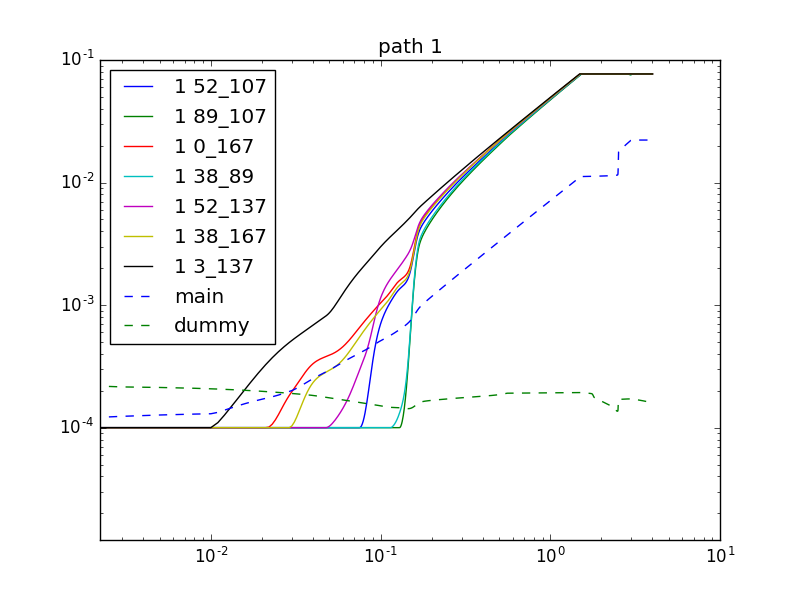
\includegraphics[width= 1 \columnwidth]{Images/Chapter5/path_1.png}
\caption{\fontsize{12pt}{11pt}\selectfont \textit{All the junctions in the main path between terminals. Main and dummy conductance shown in dotted lines}}
\label{fig: dummy_current_junctions}
\end{figure}


\section{Dummy current}
\begin{figure}[htbp]
\centering
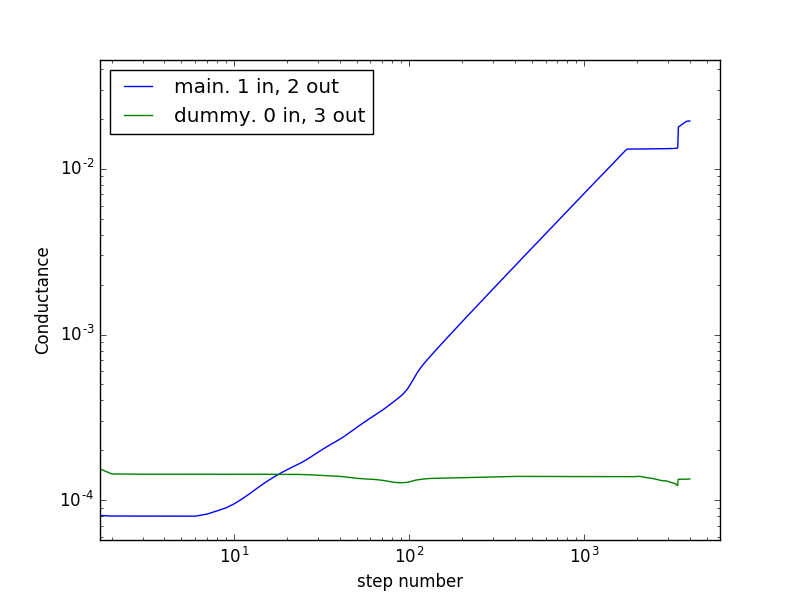
\includegraphics[width= 1 \columnwidth]{Images/Chapter5/min_1_mout_2.png}
\caption{\fontsize{12pt}{11pt}\selectfont \textit{Current is ramped up between the main electrodes, a small amount of current is extracted from the dummy terminals.}}
% Image from /home/colin/Dropbox (CRANN)/PhD/model/multi_terminal/4_terminal_pump_probe/1.1_exponent
\label{fig: dummy_current_main}
\end{figure}

A regular current scan occurs between two of the terminals, a small amount of current is passed in and out of the remaining two terminals. The conductance between the two dummy electrodes is also shown in Figure \ref{fig: dummy_current_main}. Two areas of note can be seen in the dummy conductance, namely the dip just before the PL regime in the main conductance curve and just at the end of the first plateau. In order to understand these features it is neccesary to examine the conductance of each individual junction in the main conductive path. These are shown in Fig \ref{fig: dummy_current_junctions}

\begin{figure}[htbp]
\centering
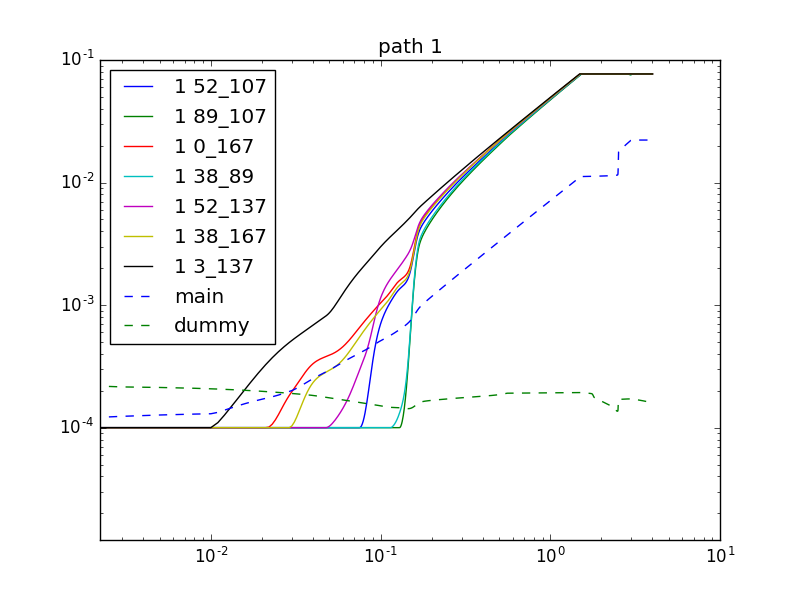
\includegraphics[width= 1 \columnwidth]{Images/Chapter5/path_1.png}
\caption{\fontsize{12pt}{11pt}\selectfont \textit{All the junctions in the main path between terminals. Main and dummy conductance shown in dotted lines}}
% Image from /home/colin/Dropbox (CRANN)/PhD/model/multi_terminal/4_terminal_pump_probe/1.1_exponent
\label{fig: dummy_current_junctions}
\end{figure}



The movement in the dummy current coincides with an initial period of conductance evolution in the junctions of the main conductive path between the main electrodes. This activity has a knock-on which manifests in the conductance of the dummy electrodes.

\section{Commutability and associativity}
It is clear from Figure \ref{fig: multi_pair_check} that the training of one path has an impact on the conductance state of other terminal pairs. Another examination for this is two test the commutability of training memory states in a NWN. First a conductance scan is performed on one pair of terminals. Any junctions that have reached an on state are fixed at this conductance value, any other conductances are allowed to reset to the off conductance state. In the case of two independant paths, i.e no terminal is used in both paths, one sees a definite commutability of memory states. The formation of one of the paths in this network has little effect on the formation of the second path. There is a slight difference in behaviour at the start of conductance scan but the latter behaviour, particularly the PL and plateau behaviour is the same for both scans. 
\begin{figure}[htbp]
\centering
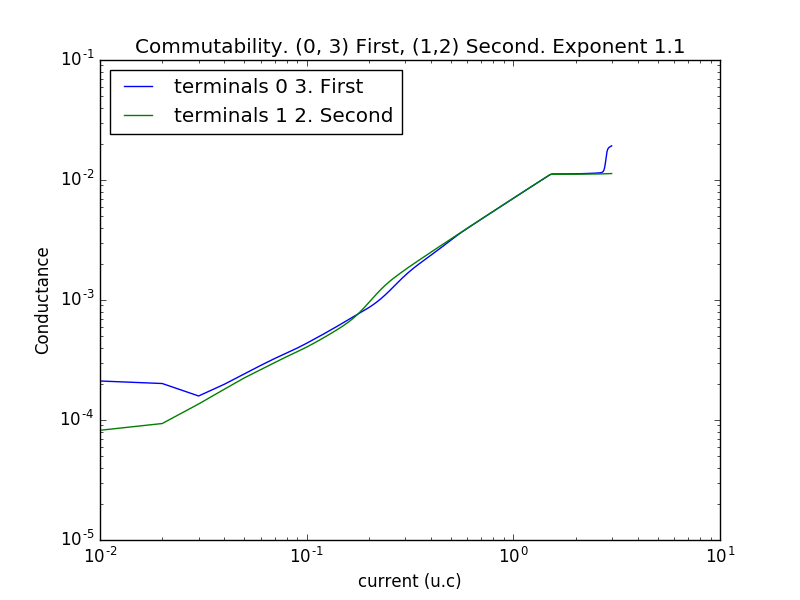
\includegraphics[width= 0.49 \columnwidth]{Images/Chapter5/0_3_f_1_2_s_expon_1_1.png}
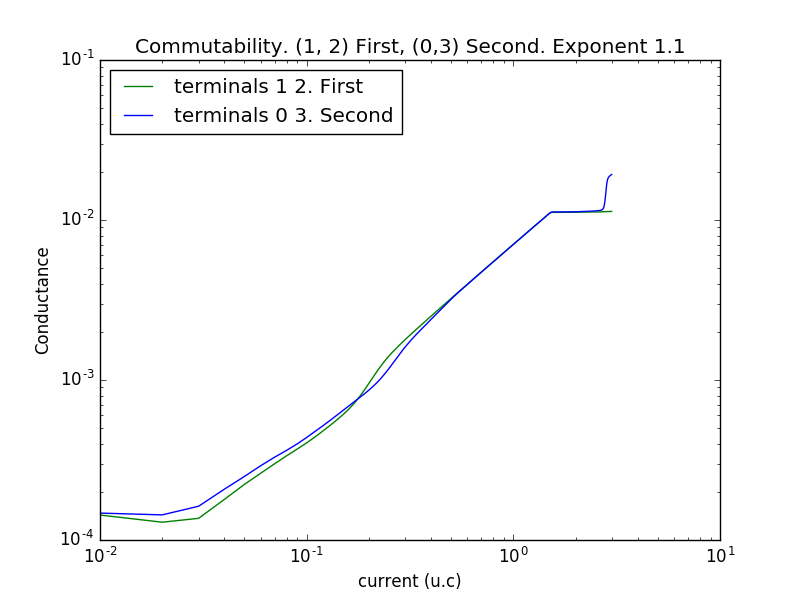
\includegraphics[width= 0.49 \columnwidth]{Images/Chapter5/1_2_f_0_3_s_expon_1_1.png}
\caption{\fontsize{12pt}{11pt}\selectfont \textit{Commutability }}
% Image from /home/colin/Dropbox (CRANN)/PhD/model/multi_terminal/commutability/density_0.5/network_1/network_1_seed_0_no_update
\label{fig: commutability}
\end{figure}
Figure \ref{fig: Associativity} shows the effect of a shared electrode on the commutability of path formation. There is a clear effect of the order of training on the final conductance states of the paths. The plot of the difference of the two conductance curves best illustrates this. These simulations highlight the effect of independent and shared terminal paths. An application of these different terminal layouts are as independent memory states, in the case the first case, and as associative memory in the latter.
\todo{add in plot of first scan - second scan}
\begin{figure}[htbp]
\centering
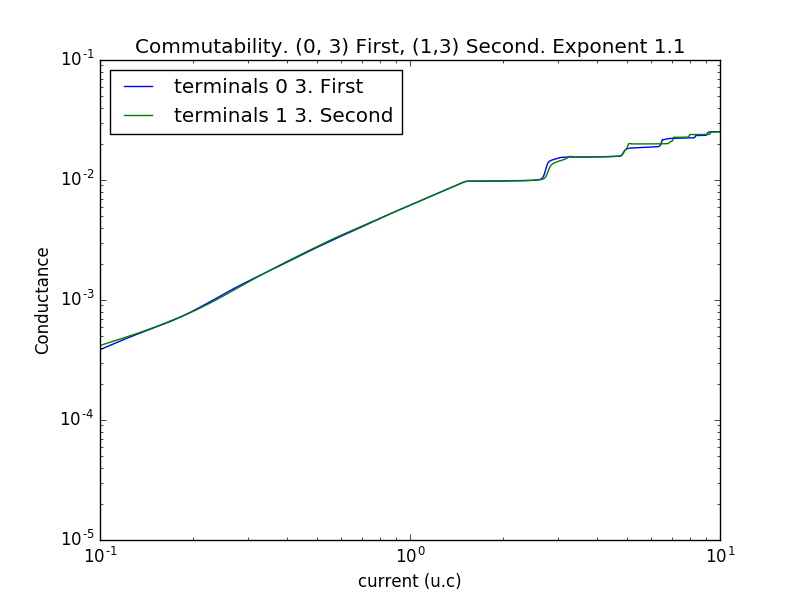
\includegraphics[width= 0.49 \columnwidth]{Images/Chapter5/associative_0_3_f_1_3_s_expon_1_1.png}
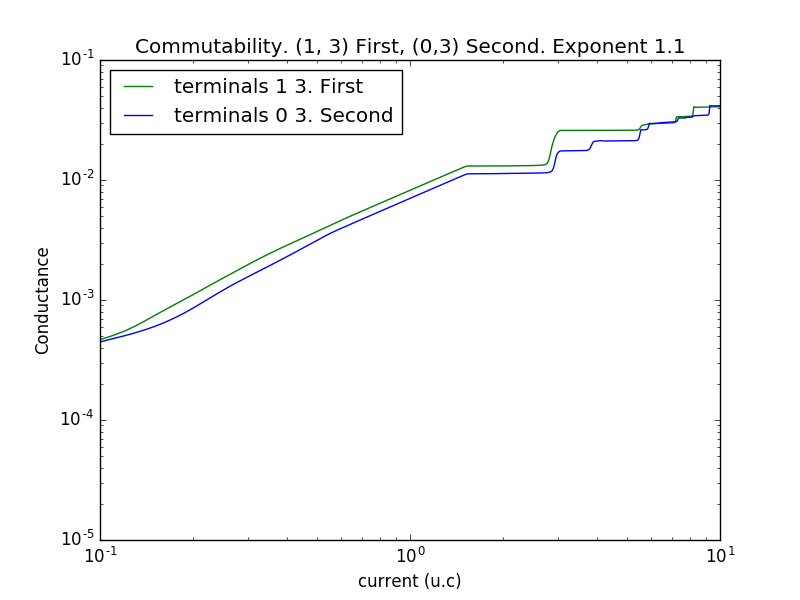
\includegraphics[width= 0.49 \columnwidth]{Images/Chapter5/associative_1_3_f_0_3_s_expon_1_1.png}
\caption{\fontsize{12pt}{11pt}\selectfont \textit{Commutability }}
% Image from /home/colin/Dropbox (CRANN)/PhD/model/multi_terminal/commutability/density_0.5/network_1/network_1_seed_0_no_update
\label{fig: Associativity}
\end{figure}
\end{comment}

%\bibliographystyle{ieeetr}  %%for ordered citations
%\bibliography{bibliography}
